\documentclass[a4paper,14pt]{extarticle}
\usepackage{cmap}
\usepackage[T2A]{fontenc}
\usepackage[utf8]{inputenc}
\usepackage[russian]{babel}
\usepackage[left=30mm,right=15mm,top=20mm,bottom=23mm]{geometry}
\usepackage{setspace}
\usepackage{indentfirst}
\usepackage{amsmath}
\usepackage{booktabs,tabularx}
\usepackage{graphicx}
\usepackage{listings}
\usepackage{xcolor}
\usepackage{caption}
\usepackage[hidelinks,unicode]{hyperref}

\onehalfspacing
\setlength{\parindent}{1.25cm}
\setlength{\emergencystretch}{1em}
\setlength{\headheight}{0pt}
\brokenpenalty=10000
\pagestyle{plain}
\captionsetup{font=small,labelsep=endash}
\captionsetup[table]{position=top}
\renewcommand{\lstlistingname}{Листинг}
\lstset{
  basicstyle=\ttfamily\small,
  numbers=left,
  numberstyle=\ttfamily\scriptsize\color{black!55},
  xleftmargin=1.4em,
  numbersep=0.7em,
  columns=fullflexible,
  keepspaces=true,
  breaklines=true,
  showstringspaces=false,
  captionpos=b,
  frame=single,
  rulecolor=\color{black!25}
}
\hypersetup{
  pdftitle={Лабораторная работа № 2. Захват и анализ сетевого трафика},
  pdfauthor={Храмов В. Д.},
  pdfsubject={Сети ЭВМ и телекоммуникации компьютерных сетей. Вариант 22}
}

\begin{document}

\begin{titlepage}
  \thispagestyle{empty}
  \begin{center}
    \begin{singlespace}
      МИНИСТЕРСТВО НАУКИ И ВЫСШЕГО ОБРАЗОВАНИЯ\\
      РОССИЙСКОЙ ФЕДЕРАЦИИ\par\medskip
      Санкт-Петербургский политехнический университет Петра Великого\par\medskip
      Институт компьютерных наук и кибербезопасности\\
      Высшая школа технологий искусственного интеллекта\\
      Направление 02.03.01 «Математика и компьютерные науки»
    \end{singlespace}

    \vfill
    {\Large\bfseries Отчёт о выполнении\\лабораторной работы №~2\par}
    \medskip
    {\large Захват и анализ сетевого трафика\par}
    \medskip
    Дисциплина «Сети ЭВМ и телекоммуникации компьютерных сетей»\par
    Вариант 22\par
  \end{center}

  \vfill
  \noindent Выполнил студент группы 5130201/40101\hfill
  \underline{\hspace{2.3cm}}\enspace Храмов В.~Д.\par\medskip
  \noindent Проверил, к.\,т.\,н.\hfill
  \underline{\hspace{2.3cm}}\enspace Мулюха В.~А.\par\medskip
  \begin{flushright}
    «\underline{\hspace{0.9cm}}» \underline{\hspace{2.6cm}} 2026 г.
  \end{flushright}

  \vfill
  \begin{center}
    Санкт-Петербург\\2026
  \end{center}
\end{titlepage}

\setcounter{page}{2}
\tableofcontents
\clearpage

\section{Цель и постановка задачи}

Цель работы --- освоить захват трафика и выделить пакеты, вызванные действиями из таблицы~\ref{tab:targets}. По заданию~\cite{assignment} требовалось сохранять как минимум первые 100--120 байт каждого пакета.

\begin{table}[htbp]
  \centering
  \caption{Адреса для варианта 22}
  \label{tab:targets}
  \begin{tabularx}{\linewidth}{@{}X l@{}}
    \toprule
    Действие & Доменное имя \\
    \midrule
    Проверка доступности с помощью \texttt{ping} & \texttt{masspinger.org} \\
    Трассировка маршрута с помощью \texttt{traceroute} & \texttt{uptrends.com} \\
    Открытие сайта в браузере & \texttt{pingwebsite.com} \\
    \bottomrule
  \end{tabularx}
\end{table}

\section{Теоретические сведения}

\subsection{Захват пакетов и измерение времени}

Программа \texttt{tcpdump} записывает пакеты с сетевого интерфейса и присваивает им отметки времени. Параметр \textit{snaplen} задаёт максимальное число сохраняемых байтов на пакет~\cite{tcpdump}. Фильтры отображения Wireshark выделяют пакеты по адресам, номерам кадров и полям протоколов~\cite{wireshark}.

\subsection{Принципы работы ping и traceroute}

Команда \texttt{ping} отправляет ICMP Echo Request (тип 8) и ожидает Echo Reply (тип 0). Пакеты сопоставляются по идентификатору и номеру последовательности. RTT (\textit{Round-Trip Time}) --- интервал между отправкой запроса и получением ответа~\cite{icmp}.

В macOS \texttt{traceroute} по умолчанию отправляет UDP-пробы с последовательно возрастающим TTL (\textit{Time to Live})~\cite{traceroute}. При пересылке маршрутизатор уменьшает TTL. Когда значение исчерпано, маршрутизатор отбрасывает пробу и может вернуть ICMP Time Exceeded (тип 11, код 0). Сообщение содержит начало исходной пробы, чтобы его можно было сопоставить с конкретным UDP-пакетом~\cite{icmp}. При достижении конечного узла с закрытым UDP-портом возможен ответ ICMP Port Unreachable (тип 3, код 3).

\subsection{Разрешение имени и защищённое соединение}

DNS преобразует доменное имя в сетевые адреса. Записи \texttt{A} содержат адреса IPv4, а \texttt{AAAA} --- IPv6. При HTTPS поверх TCP сначала устанавливается TCP-соединение обменом \texttt{SYN}, \texttt{SYN, ACK} и \texttt{ACK}~\cite{tcp}. Затем клиент отправляет \textit{Client Hello}, а сервер отвечает \textit{Server Hello} с согласованными параметрами TLS. Имя сайта может быть видно в расширении SNI (\textit{Server Name Indication}) сообщения \textit{Client Hello}. HTTP-обмен передаётся в зашифрованном виде~\cite{tls}.

\section{Порядок выполнения}

Захват выполнен 22 ноября 2026 г. на MacBook Air под управлением macOS. Команда просмотра маршрута IPv4 по умолчанию показала интерфейс \texttt{en0}. В первом окне Терминала на этом интерфейсе был запущен \texttt{tcpdump}. Во втором окне последовательно были выполнены действия из листинга~\ref{lst:commands}. В журнале~\cite{commandlog} отмечено время начала каждого действия по московскому времени. После обращения к сайту захват был остановлен сочетанием \texttt{Ctrl+C}.

\begin{lstlisting}[caption={Команды захвата и генерации трафика},label={lst:commands}]
route -n get default | awk '$1 == "interface:" {print $2}'
sudo tcpdump -i en0 -p -s 0 -w "lab2-22-$(date +%Y%m%d-%H%M%S).pcap"

ping -n -c 4 -t 12 masspinger.org
traceroute -n -m 30 -w 2 uptrends.com
open 'https://pingwebsite.com'
\end{lstlisting}

В файле захвата~\cite{capture} содержится 33\,949 кадров Ethernet. Первый кадр зарегистрирован в 16:00:23, последний --- в 16:06:41. Установленный лимит составил 524\,288 байт на пакет. При сверке исходной и сохранённой длин всех кадров усечений не обнаружено. По итоговому выводу \texttt{tcpdump} ядро не отбросило ни одного пакета при захвате.

\section{Результаты и анализ}

\subsection{Проверка доступности masspinger.org}

Для \texttt{masspinger.org} получен IPv4-адрес \texttt{104.21.22.170}. В захвате были выделены четыре Echo Request и четыре Echo Reply. У всех пакетов совпал идентификатор \texttt{0xa84d}. Каждая пара запроса и ответа сопоставлена по номеру последовательности. Например, кадр 507 содержит запрос с номером 2, а кадр 520 --- ответ с тем же номером. По отметкам захвата получено
\[
  RTT = t_{520} - t_{507}
      = 7{,}517173 - 7{,}445725
      = 0{,}071448\,\text{с} = 71{,}448\,\text{мс},
\]
где $t_{507}$ и $t_{520}$ --- время запроса и ответа в секундах от начала записи.

\begin{table}[htbp]
  \centering
  \caption{Сопоставление запросов и ответов ICMP}
  \label{tab:ping}
  \begin{tabular}{@{}r r r r r@{}}
    \toprule
    Номер & Запрос & Ответ & RTT по захвату, мс & RTT по \texttt{ping}, мс \\
    \midrule
    0 & 259 & 262 & 172,500 & 173,030 \\
    1 & 336 & 349 & 135,534 & 135,888 \\
    2 & 507 & 520 & 71,448 & 71,824 \\
    3 & 774 & 777 & 81,700 & 82,212 \\
    \bottomrule
  \end{tabular}
\end{table}

По данным таблицы~\ref{tab:ping}, средний RTT по захвату составил 115,296 мс, а по журналу команды --- 115,739 мс. Эти значения получены из двух наборов отметок времени: на сетевом интерфейсе и в утилите. На каждый из четырёх запросов получен ответ, поэтому доля потерь в опыте составила 0\,\%.
\clearpage

\subsection{Трассировка маршрута до uptrends.com}

Адрес назначения в выводе \texttt{traceroute} --- \texttt{178.162.193.241}. Зарегистрировано 90 исходящих UDP-проб: по три на каждое значение TTL от 1 до 30. UDP-порт отправителя был равен 52653, а порт назначения менялся от 33435 до 33524.

В кадре 780 зафиксирована первая проба с TTL~1 и UDP-портом назначения 33435. В ответном кадре 781 внешний заголовок IPv4 указывает на отправителя \texttt{172.20.10.1}, а поля ICMP содержат тип~11 и код~0. Во вложенных заголовках ответа сохранены адрес назначения \texttt{178.162.193.241} и порты 52653 и 33435. Совпадение этих полей связывает ответ с пробой 780. По отметкам кадров задержка до первого узла и обратно составила 3,937 мс.

\begin{table}[htbp]
  \centering
  \caption{Ответившие узлы по данным traceroute и захвата}
  \label{tab:trace}
  \begin{tabularx}{\linewidth}{@{}r X l r@{}}
    \toprule
    TTL пробы & Адреса отправителей ICMP & Кадры ответов & Ответов \\
    \midrule
    1  & \texttt{172.20.10.1} & 781, 783, 785 & 3 \\
    10 & \texttt{80.81.194.12} & 7622, 7724, 7934 & 3 \\
    11 & \texttt{31.31.34.225}, \texttt{31.31.34.221} & 8316, 8950, 9819 & 3 \\
    12 & \texttt{212.95.37.79}, \texttt{212.95.37.81} & 10208, 10210 & 2 \\
    \bottomrule
  \end{tabularx}
\end{table}

В таблице~\ref{tab:trace} приведены все 11 ответов ICMP на снятые пробы. На переходах 2--9 и 13--30 вывод содержал по три звёздочки, а на переходе 12 --- одну. Каждая звёздочка соответствует пробе, на которую ответ не был получен за 2~с. Ответы на пробах с TTL~10 показывают, что пакеты продолжали проходить после переходов 2--9. Последние ответы получены на пробах с TTL~12. Достижение адреса назначения в этой трассировке не подтверждено.
\clearpage

\subsection{Доступ к pingwebsite.com в браузере}

После запуска браузера в 16:03:11 зафиксированы три DNS-запроса к \texttt{pingwebsite.com}. Они отправлены по UDP на порт~53 через локальный DNS-сервер \texttt{172.20.10.1}. Кадры запроса и ответа и основные результаты приведены в таблице~\ref{tab:dns}.

\begin{table}[htbp]
  \centering
  \caption{DNS-обмен для pingwebsite.com}
  \label{tab:dns}
  \begin{tabularx}{\linewidth}{@{}l r r >{\raggedright\arraybackslash}X@{}}
    \toprule
    Тип & Запрос & Ответ & Результат \\
    \midrule
    \texttt{A} & 15352 & 15403 & \texttt{104.21.10.244}, \texttt{172.67.131.189} \\
    \texttt{AAAA} & 15351 & 15413 & \texttt{2606:4700:3031::ac43:83bd}, \texttt{2606:4700:3030::6815:af4} \\
    \texttt{HTTPS} & 15350 & 15930 & Параметры HTTPS-сервиса \\
    \bottomrule
  \end{tabularx}
\end{table}

Запрос и ответ \texttt{AAAA} имеют один идентификатор DNS-транзакции \texttt{0x3aa6}. Между этими кадрами прошло 151,192 мс. В первом зафиксированном HTTPS-соединении браузер использовал адрес \nolinkurl{2606:4700:3031::ac43:83bd} из этого ответа. Начало TCP- и TLS-обмена показано на рисунке~\ref{fig:browser}. В кадрах 15441, 15523 и 15525 наблюдается TCP-рукопожатие между портом клиента 62089 и портом сервера 443.

\begin{figure}[htbp]
  \centering
  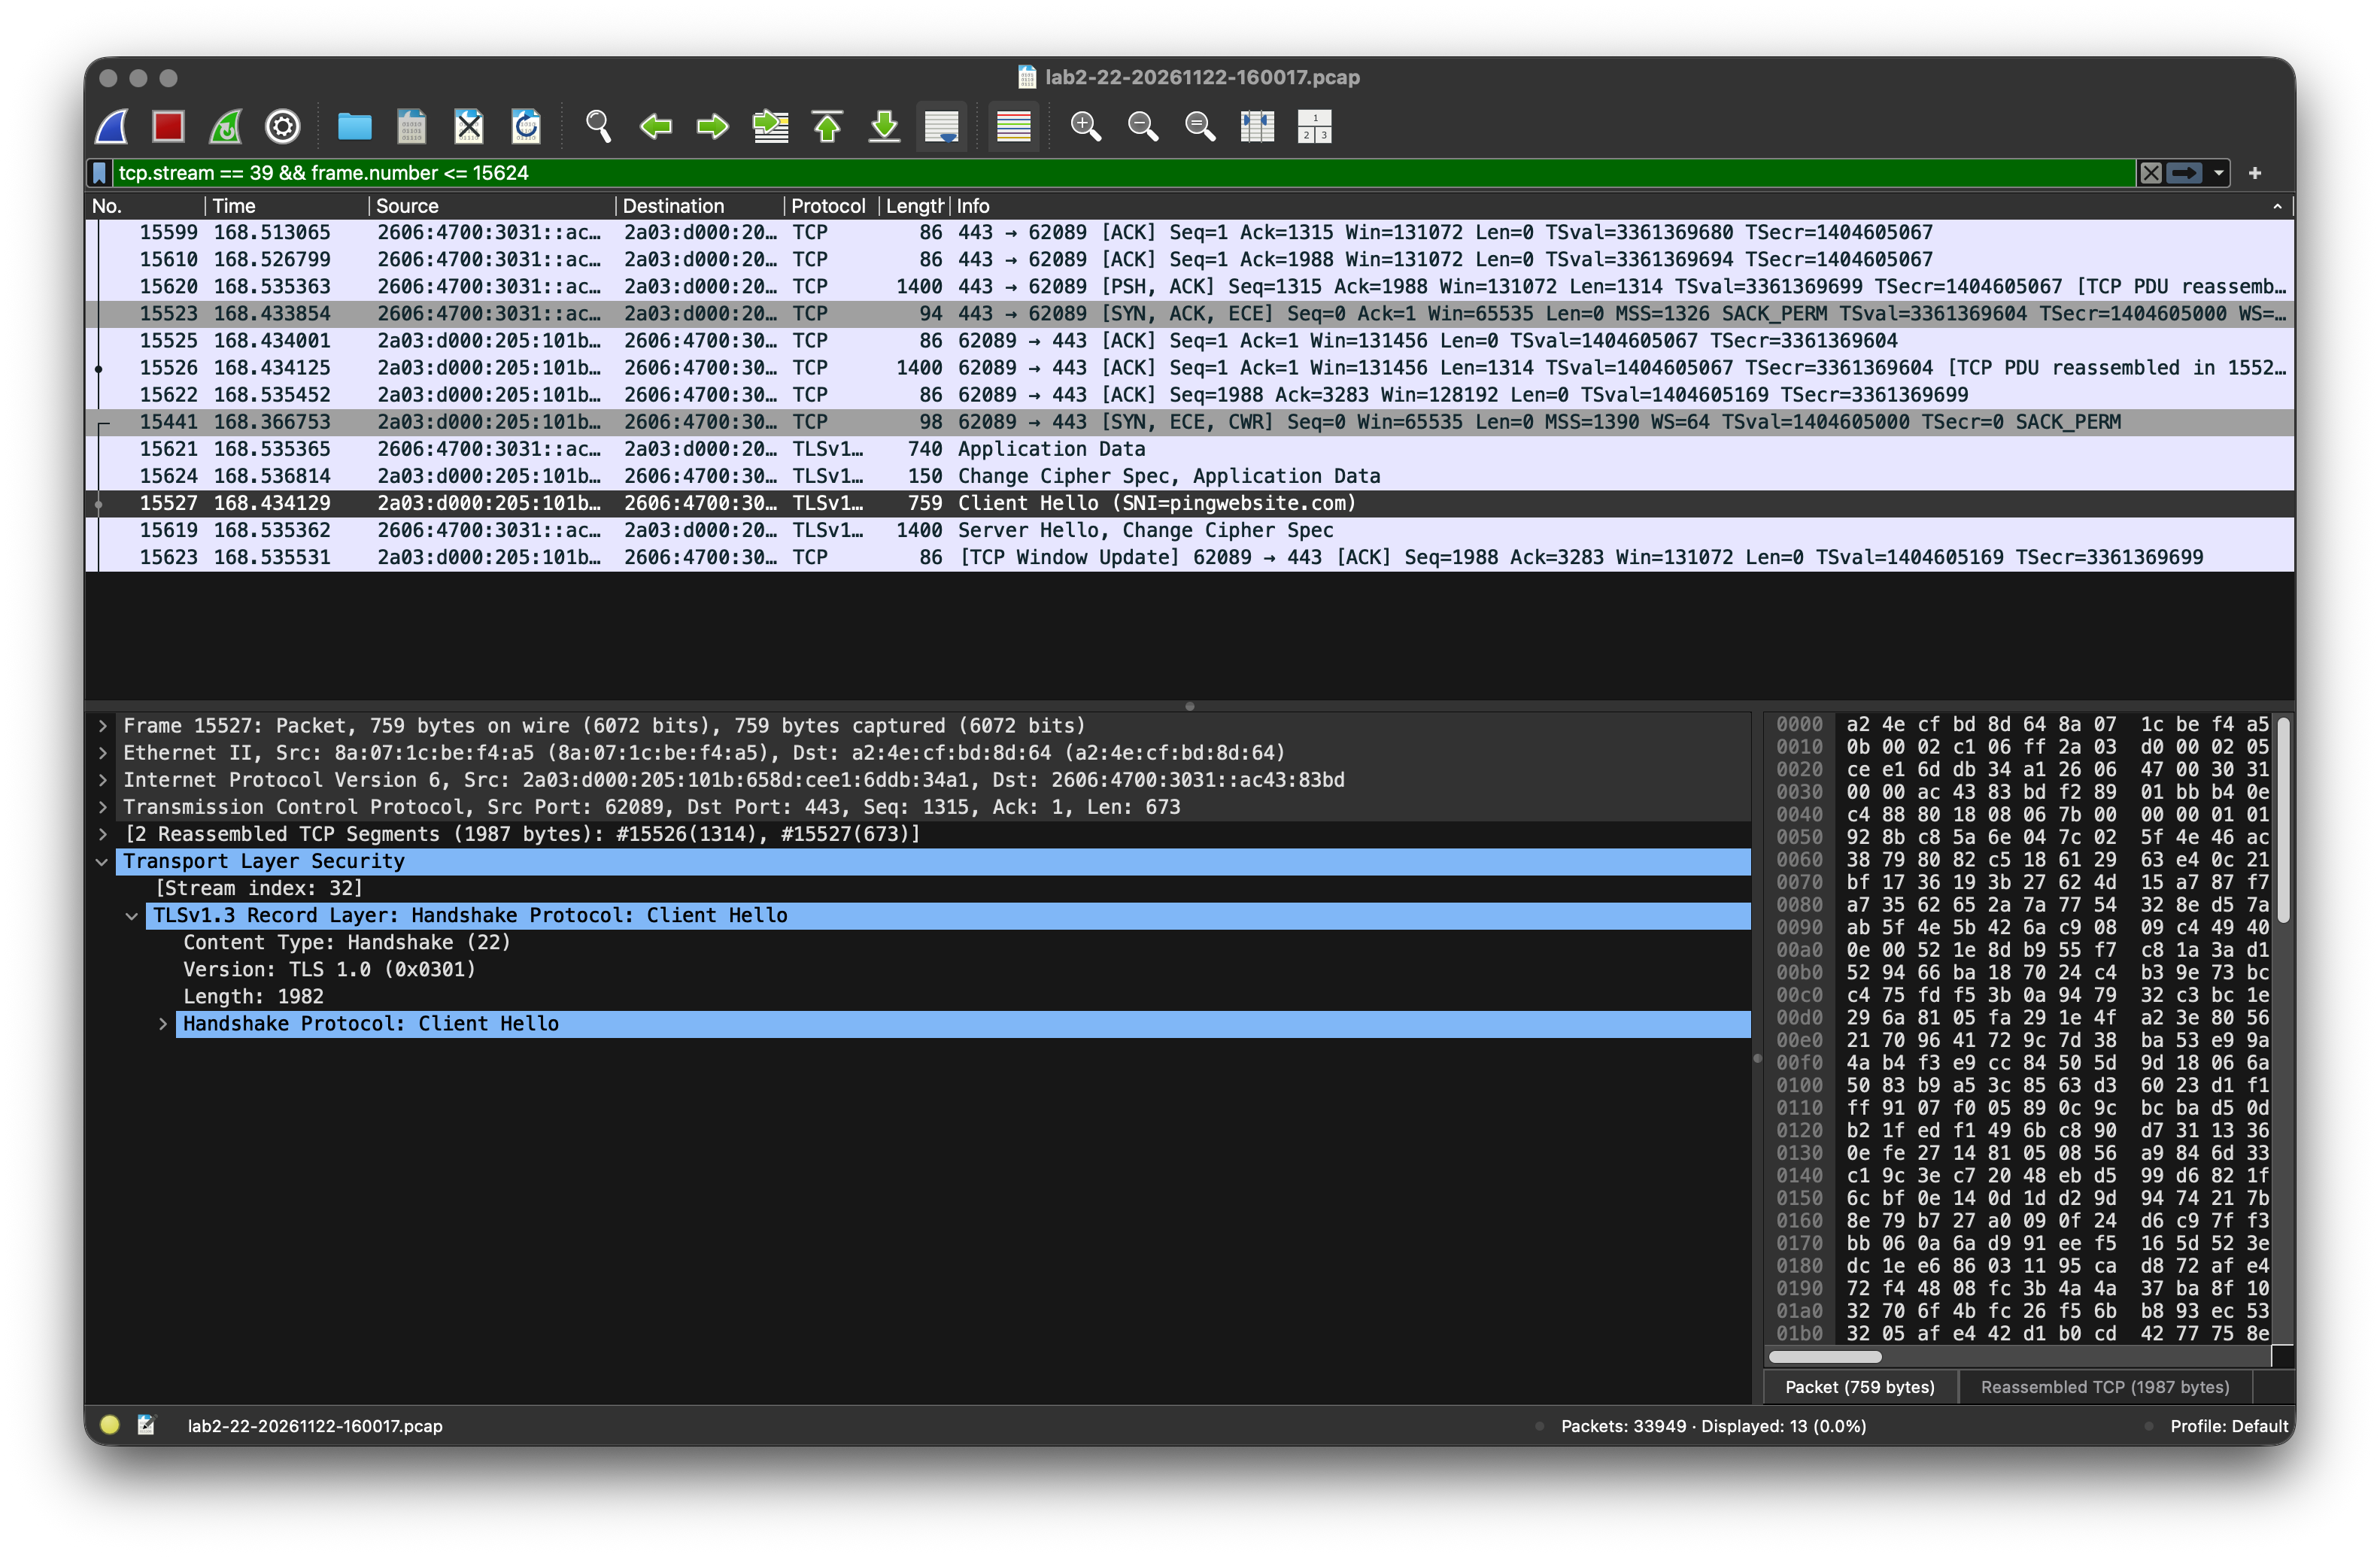
\includegraphics[width=\linewidth,viewport=56bp 546bp 1410bp 997bp,clip]{images/browser-client-hello.png}
  \caption{Начальные кадры TCP и TLS в Wireshark}
  \label{fig:browser}
\end{figure}

Wireshark собрал \textit{Client Hello} из TCP-сегментов в кадрах 15526 и 15527. В сообщении видно имя \texttt{pingwebsite.com} в расширении SNI. Кадр 15619 содержит \textit{Server Hello}, в котором сервер указал версию TLS~1.3. Затем наблюдаются зашифрованные записи TLS в обоих направлениях, в том числе в кадрах 15621 и 15624. Сайт во время записи загружался долго. При отдельном посещении в браузере отобразились диаграммы.
\clearpage

\section{Заключение}

В захвате выделены пакеты всех трёх действий. При проверке \texttt{masspinger.org} получены четыре ответа ICMP из четырёх. При трассировке \texttt{uptrends.com} UDP-пробы были сопоставлены с сообщениями ICMP Time Exceeded, что позволило определить ответившие промежуточные узлы. Для \texttt{pingwebsite.com} прослежена последовательность от разрешения имени DNS до TCP-соединения по IPv6 и обмена записями TLS~1.3. Выделение пакетов подтверждено их номерами, адресами и полями соответствующих протоколов.

\renewcommand{\refname}{Список источников}
\phantomsection
\addcontentsline{toc}{section}{Список источников}
\begin{thebibliography}{9}
  \raggedright
  \bibitem{assignment} Задание к лабораторной работе №~2 и таблица вариантов. Файл \nolinkurl{task.md}.
  \bibitem{commandlog} Журнал команд для варианта 22. Файл \nolinkurl{lab2-22-commands-20261122-160028.txt}.
  \bibitem{capture} Захват на интерфейсе \texttt{en0} от 22 ноября 2026 г. Файл \nolinkurl{lab2-22-20261122-160017.pcap}.
  \bibitem{tcpdump} Apple. \href{https://github.com/apple-oss-distributions/tcpdump/blob/main/tcpdump/tcpdump.1}{Справочная страница tcpdump}.
  \bibitem{wireshark} Wireshark Foundation. \href{https://www.wireshark.org/docs/wsug_html_chunked/ChWorkDisplayFilterSection.html}{Руководство пользователя, фильтры отображения}.
  \bibitem{icmp} Postel J. \href{https://www.rfc-editor.org/rfc/rfc792.html}{Internet Control Message Protocol}. RFC 792, 1981.
  \bibitem{traceroute} Apple. \href{https://github.com/apple-oss-distributions/network_cmds/blob/main/traceroute.tproj/traceroute.8}{Справочная страница traceroute}.
  \bibitem{tcp} Eddy W. \href{https://www.rfc-editor.org/rfc/rfc9293.html}{Transmission Control Protocol (TCP)}. RFC 9293, 2022.
  \bibitem{tls} Rescorla E. \href{https://www.rfc-editor.org/rfc/rfc8446.html}{The Transport Layer Security (TLS) Protocol Version 1.3}. RFC 8446, 2018.
\end{thebibliography}

\end{document}
